\chapter{System Analysis}
\section{Requirement elicitation}
\subsection{Stakeholders}
\begin{itemize}
    \item End users: tenants, landlords
    \item System owner: Ho Chi Minh City University of Technology
\end{itemize}
\subsection{Functional Requirements}
\begin{enumerate}
    \item Tenant
    \begin{itemize}
        \item The tenant can ask the chatbot to search for available rental listings based on places or neighborhoods. 
        \item The tenant can compare between 2 properties' information
        \item The tenant can filter available rental listings based on location, amenities, area, price, room type or specific keywords.
        \item The tenant can see the details of rental posts: accurate property listings with high-quality photos, comprehensive descriptions of the property and information about landlords.
        \item The tenant can save listings to a favorites shortlist so that the tenant can compare and revisit these properties later.
        \item The tenant can chat or contact the owner directly on the site.
        \item The tenant can verify property owner identities, conduct background checks, and review rental histories.
        \item The tenant can receive notifications about responses from the property owner, rental visits or any updates related to the rental application.
    \end{itemize}
    
    \item Landlord (property owner)
    \begin{itemize}
        \item The landlord can create and manage his/her rental property listing.
        \item The landlord can provide details information about the property.
        \item The landlord can ask the chat-bot system to create or manage rental property for them
        \item The landlord can verify tenant identities, conduct background checks, and review rental histories.
        \item The landlord can see the list of people who are interested in the property in their rental listings.
        \item The landlord can receive notifications about contact from tenant
        \item The landlord can chat or contact with tenant directly on the site
    \end{itemize}
    \item Others
    \begin{itemize}
        \item The system can get more rental data from the internet (other real-estate websites) and display on the system website.
        \item The system can provide related rental property based on the rental that the tenant is interested in.
        \item The system must be able to understand questions, and answer the questions from user in Vietnamese.
        \item The system must send notifications to the tenant about updated information in their favorite rental list.
    \end{itemize}
\end{enumerate}


\subsection{Non-functional Requirements}
\begin{enumerate}
    \item Usability
    \begin{itemize}
        \item The system has a user-friendly interface that the users can know how to use in less than 2 minutes.
        \item Tenant use and Landlord use should be clearly separated on the website.
    \end{itemize}
    \item Performance
    \begin{itemize}
        \item The system is able to process multiple (1000) users at a time.
        \item The system response time is less than 3 seconds.
        \item Search result accuracy should be at least 90\%.
        \item Unable to search response is less than 5\%.
        \item Beside the filter, the system can allow the user to search with natural language in the search engine
    \end{itemize}
    \item Security
    \begin{itemize}
        \item User conversations and account information must be protected.
    \end{itemize}
    \item Portability and compatibility
    \begin{itemize}
        \item The system should be compatible with three screen sizes (mobile, tablet, and desktop).
    \end{itemize}
    \item Development
    \begin{itemize}
        \item The system can be extendable to add more functions.
        \item The system can be extendable to process English.
    \end{itemize}
\end{enumerate}


\newpage
\section{Use case specification}
% short intro
Before using the application, user must sign up or log in with an account. Therefore, the requirement for Authentication and Authorization is already considered in the system, we will implement the Authentication module but not demonstrate it in the use-case diagrams for convenience. That way, we can pay more attention to the other modules. However, we must explain the authenticated flow in detail in activity diagrams because of some constraints that end-users of this website have to follow when use the apps. The main application, we call it Rental System, composes the features corresponding to 2 types of end-users: Tenant and Landlord. 

% %%%%%%%%% Rental system: Tenant view %%%%%%%%%%
\subsection{Rental system: Tenant view}
\subsubsection{Use case diagram}
\begin{figure}[H]
    \centering
    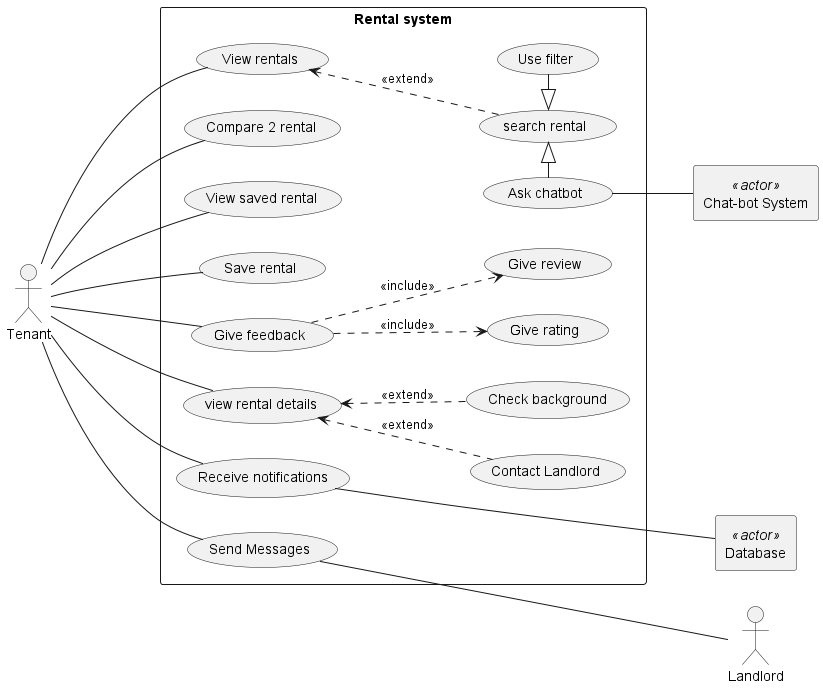
\includegraphics[width = 0.9\textwidth]{Images/rental_system_tenant.png}
    \caption{Use Case diagram: Rental System in Tenant view}
    \label{fig:enter-label}
\end{figure}

% %%%%%%%%%%%%%%%%%%%% Use case scenarios %%%%%%%%%%
\newpage
\subsubsection{Use-case Scenarios}

%%%----UC-01-------
\begin{table}[H]
    \centering
% \usepackage{tabularray}
\begin{longtblr}[
  label = none,
  entry = none,
]{
  width = \linewidth,
  colspec = {Q[140]Q[802]},
  hlines,
  vlines,
}
\textbf{Use-case ID}       & UC-01               \\
\textbf{Use-case Name}     & View rentals        \\
\textbf{Actor(s)}          & Tenant (Primary), Chat-bot System (Secondary)    \\
\textbf{Description}       & Tenant can see all the rentals general information in the main page or search page of application                    \\
\textbf{Pre-condition(s)}  & Tenant accesses to the website                                     \\
\textbf{Post-condition(s)} & The rentals listing will be shown on the main page of website        \\
\textbf{Trigger(s)}        & User is on the main page or search page                              \\
\textbf{Normal flow}       & {1. System display the list of available rentals on the page\\2. User scroll the page for more rentals\\3. System display rentals}                                 \\
\textbf{Alternative flow}  & {Alternative 1: at step 2\\ 2.1a. User choose the chat-bot to narrow down the list\\ 2.1b. System open the chat-bot\\ 2.1c. User search for rental using the chat-bot module (this will be explained with more details in use cases for chat-bot system)\\ 2.1d. Chat-bot return search result\\ Continue at step 3 of normal flow\\Alternative 2: at step 2\\  2.2a. User choose the filter to narrow down the list\\  2.2b. System open the filtering form\\  2.2c. User search for rental by completing and submitting the form\\  2.2d. System search for result\\ Continue at step 3 of normal flow} \\
\textbf{Exception flow}    & {Exception 1: No result found at step 2.1d or 2.2d\\ - If no rental information matches the requirement, then the system display "No rental result found" message to the tenant}                           \end{longtblr}
    \caption{Use case scenario: View list available rentals}
    \label{tab:usecase-scenario-view-rentals}
\end{table}



%%%----UC-02-------
\newpage
% \usepackage{tabularray}
\begin{table}[H]
    \centering
\begin{longtblr}[
  label = none,
  entry = none,
]{
  width = \linewidth,
  colspec = {Q[130]Q[797]},
  hlines,
  vlines,
}
\textbf{Use-case ID}       & UC-02               \\
\textbf{Use-case Name}     & View rental detail  \\
\textbf{Actor(s)}          & Tenant (Primary)    \\
\textbf{Description}       & Tenant can see all the rentals detail information                   \\
\textbf{Pre-condition(s)}  & User see the list of rentals in main page or search page           \\
\textbf{Post-condition(s)} & Tenant can see all the rentals detail information (accurate property listings with high-quality photos, comprehensive descriptions of the property and information about landlord)                      \\
\textbf{Trigger(s)}        & Tenant clicks on a rental post in the list of rental                \\
\textbf{Normal flow}       & {1. System routes to rental detail page
\\2. System display detail information about the rental
\\3. User return to the main page
\\4. System routes to the main page
\\End use case}                                  \\
\textbf{Alternative flow}  & {Alternative 1: at step 2 - Tenant want to check Landlord background
\\ 2.1a. Tenant click on Landlord Title in Landlord section
\\ 2.1b. System routes to Landlord detail page (more information: title, time register, reviews, ratings, related rental properties, contact information)
\\ 2.1c. User return to the rental detail page
\\ 2.2d. System routes to rental detail page
\\ Continue at step 3 of normal flow
\\Alternative 2: at step 2 or 2.1b - Tenant want to contact the Landlord
\\ 2.2a. Tenant clicks on Landlord contact button
\\ 2.2b. System open the message section
\\ 2.2c. User start sending message or calling
\\ 2.2d. User closes the message section
\\ 2.2e. User return to the rental detail page
\\ 2.2f. System routes to rental detail page
\\ Continue at step 3 of normal flow } \\
\textbf{Exception flow}    & No exception        \end{longtblr}
    \caption{Use case scenario: View rental detail information}
    \label{tab:usecase-scenario-view-rental-detail}
\end{table}              


%%%----UC-03-------
\newpage
\begin{table}[H]
    \centering
\begin{longtblr}[
  label = none,
  entry = none,
]{
  width = \linewidth,
  colspec = {Q[215]Q[727]},
  hlines,
  vlines,
}
\textbf{Use-case ID}       & UC-03                            \\
\textbf{Use-case Name}     & Compare 2 rentals                \\
\textbf{Actor(s)}          & Tenant (Primary)                 \\
\textbf{Description}       & Tenant can compare 2 rentals side by side                                                  \\
\textbf{Pre-condition(s)}  & Tenant see the list of rentals in main page or search page                                      \\
\textbf{Post-condition(s)} & The system show the information of 2 rental post side by side                                 \\
\textbf{Trigger(s)}        & Tenant clicks on "compare" button a rental post in the list of rental~                   \\
\textbf{Normal flow}       & {1. Tenant clicks on "compare" button of a rental post\\2. Tenant clicks on other rental post in the list~\\3. System routes to Compare page\\4. System shows the information side by side\\5. Tenant might return to the main page\\End use case} \\
\textbf{Alternative flow}  & No alternative
\\
\textbf{Exception flow}    & No exception        \end{longtblr}
    \caption{Use case scenario: Compare 2 rental information}
    \label{tab:usecase-scenario-compare-2-rentals}
\end{table}


%%-----UC-04----------
\newpage
\begin{table}[H]
    \centering
\begin{longtblr}[
  label = none,
  entry = none,
]{
  width = \linewidth,
  colspec = {Q[213]Q[731]},
  hlines,
  vlines,
}
\textbf{Use-case ID}       & UC-04                      \\
\textbf{Use-case Name}     & Save rental post           \\
\textbf{Actor(s)}          & Tenant (Primary)           \\
\textbf{Description}       & Tenant can save rental post into saved list for later reviewing                \\
\textbf{Pre-condition(s)}  & User see the list of rentals in main page or on the rental detail page       \\
\textbf{Post-condition(s)} & The rentals post added to the saved list                                          \\
\textbf{Trigger(s)}        & Tenant clicks the "Heart icon" on the rental post~                               \\
\textbf{Normal flow}       & {1. Tenant on the main page (show list of rental)\\2. Tenant clicks on "Heart icon" on the rental post\\3. System added the rental post to saved list\\4. System prompt message "Rental saved"\\End use case} \\
\textbf{Alternative flow}  & {Alternative 1: at step 1 - Tenant clicks to see rental detail\\~1.1a. System routes to rental detail page\\~1.1b. Tenant clicks on SSave rental" button\\~Continue in step 3 of normal flow}                 \\
\textbf{Exception flow}    & No exception               \end{longtblr}
    \caption{Use case scenario: Save rentals to saved list}
    \label{tab:usecase-scenario-save-rentals}
\end{table}

%--------UC-05---------
\newpage
\begin{table}[H]
    \centering
% \usepackage{tabularray}
\begin{longtblr}[
  label = none,
  entry = none,
]{
  width = \linewidth,
  colspec = {Q[138]Q[804]},
  hlines,
  vlines,
}
\textbf{Use-case ID}       & UC-05                      \\
\textbf{Use-case Name}     & View saved rentals         \\
\textbf{Actor(s)}          & Tenant (Primary)           \\
\textbf{Description}       & Tenant can see list of rentals post in saved list                              \\
\textbf{Pre-condition(s)}  & User logged in successfully                                            \\
\textbf{Post-condition(s)} & The saved rentals listing will be shown on the main page of website               \\
\textbf{Trigger(s)}        & Tenant click on the "Saved rentals" button                                         \\
\textbf{Normal flow}       & {1. Tenant click on the "Saved rentals" button\\2. System displays list of saved rental post on the saved section~\\End use case}  \\
\textbf{Alternative flow}  & No alternative             \\
\textbf{Exception flow}    & {Exception 1: at step 2 - the saved list is empty\\ - If the list is empty, tenant haven't save any rental post yet , then the system display "No rental result found" message to the tenant} 
\end{longtblr}
    \caption{Use case scenario: View saved rentals}
    \label{tab:usecase-scenario-view-saved-rentals}
\end{table}


%------UC-06-----
\newpage
\begin{table}[H]
    \centering
% \usepackage{tabularray}
\begin{longtblr}[
  label = none,
  entry = none,
]{
  width = \linewidth,
  colspec = {Q[165]Q[777]},
  hlines,
  vlines,
}
\textbf{Use-case ID}       & UC-06                        \\
\textbf{Use-case Name}     & Give feedback                \\
\textbf{Actor(s)}          & Tenant (Primary)             \\
\textbf{Description}       & Tenant can give feedback on the rental post about the rental expericence or about the Landlord                                                  \\
\textbf{Pre-condition(s)}  & No precondtion               \\
\textbf{Post-condition(s)} & System updates rating and review in rental information and Landlord profile         \\
\textbf{Trigger(s)}        & Tenant click on the "Star Icon" on the rental post or the "Feedback button" on the rental detail page                                        \\
\textbf{Normal flow}       & {1. Tenant clicks on "Star Icon" on the rental post\\2. System opens a Feedback form\\3. Tenant enters rating and reviews for the rental experience\\4. Tenant enters rating and reviews for the Landlord\\5. Tenant submits the form\\6. System updates rating and review information\\7. System closes the fom and prompts message "Feedback updated"\\End use case} \\
\textbf{Alternative flow}  & {Alternative 1: at step 1 - Tenant on the rental detail page\\~1.a. Tenant scrolls to review section\\~1.b. Tenant clicks on "Leave feedback" button\\~Continue at step 2 in normal flow}               \\
\textbf{Exception flow}    & No exception                 \end{longtblr}
    \caption{Use case scenario: Tenant leave feedback on rental experience and Landlord credibility}
    \label{tab:usecase-scenario-give-feedback}
\end{table}


%-----UC-07---------
\newpage
\begin{table}[H]
    \centering
% \usepackage{tabularray}
\begin{longtblr}[
  label = none,
  entry = none,
]{
  width = \linewidth,
  colspec = {Q[196]Q[746]},
  hlines,
  vlines,
}
\textbf{Use-case ID}       & UC-07                         \\
\textbf{Use-case Name}     & Receive notification          \\
\textbf{Actor(s)}          & Tenant (Primary), Database System (Secondary)              \\
\textbf{Description}       & Tenant receives notification when there are updates information in saved list           \\
\textbf{Pre-condition(s)}  & Tenant had saved rental post to favorite list~                                          \\
\textbf{Post-condition(s)} & System send notification into Tenant notification box and email                          \\
\textbf{Trigger(s)}        & Landlord updates rental listing information                                        \\
\textbf{Normal flows}      & {1. Landlord updates information in the rental listing\\2. System updates the information into databse\\3. System publishes updates to the tenant who saved the rental\\4. Tenant receives the notification\\End use case} \\
\textbf{Alternative flow}  & No alternative                \\
\textbf{Exception flow}    & {Exception 1: \\If Tenant have not saved any rental post, then when there is an updates, no notification will be sent.}                  \end{longtblr}
    \caption{Use case scenario: Tenant receive notification about updates information}
    \label{tab:usecase-scenario-receive-information}
\end{table}


%-----UC-08-------
\newpage
\begin{table}[H]
    \centering
% \usepackage{tabularray}
\begin{longtblr}[
  label = none,
  entry = none,
]{
  width = \linewidth,
  colspec = {Q[188]Q[754]},
  hlines,
  vlines,
}
\textbf{Use-case ID}       & UC-08                       \\
\textbf{Use-case Name}     & Send messages                 \\
\textbf{Actor(s)}          & Tenant (Primary), Landlord(secondary)                                        \\
\textbf{Description}       & Tenant want to send message to Landlord                                                \\
\textbf{Pre-condition(s)}  & Tenant had account and logged in successfully  \\
\textbf{Post-condition(s)} & Tenant can contact with Landlord~                                                  \\
\textbf{Trigger(s)}        & Tenant click on "Message Icon" on rental detail post, or on Landlord profile page~  \\
\textbf{Normal flows}      & {Normal flow 1: Tenant send message to Landlord for the first time\\1. Tenant clicks on the Icon\\2. System added Landlord into contact list\\3. System opens message section\\4. Tenant enters message into chat input\\5. System sends message to correspond Landlord\\6. Tenant click on "Close Button" the message section\\7. System closes the message section\\Use case ends} \\
\textbf{Alternative flow}  & {Alternative 1: at step 6 - Landlord responses\\1.1. Tenant receives message\\Return in step 5\\Alternative 2: Tenant contact with Landlord before\\2.1. Tenant clicks on "Message Icon" on the main page\\2.2. System opens the message section with chat list\\2.3. Tenant choose the existed Landlord\\Continue at step 3 in normal flow}                                     \\
\textbf{Exception flow}    & {No exception}
\end{longtblr}
    \caption{Use case scenario: Tenant sends message to Landlord}
    \label{tab:usecase-scenario-tenant-send-message}
\end{table}


%%%%%%%%%% Rental system: Landlord %%%%%%%%%%%%%%%
\newpage
\subsection{Rental system: Landlord view}
The same as Tenant
\subsubsection{Use case diagram}
\begin{figure}[H]
    \centering
    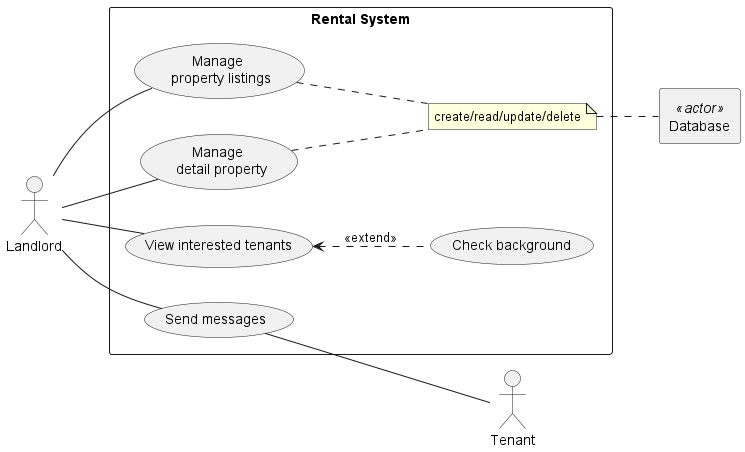
\includegraphics[width = \textwidth]{Images/rental_systen_landlord.png}
    \caption{Use Case diagram: Rental System in Landlord view}
    \label{fig:enter-label}
\end{figure}

\newpage
\subsubsection{Use case scenario}
%-------------UC-09-1---------------
\begin{table}[H]
    \centering
% \usepackage{tabularray}
\begin{longtblr}[
  label = none,
  entry = none,
]{
  width = \linewidth,
  colspec = {Q[160]Q[785]},
  hlines,
  vlines,
}
\textbf{Use-case ID}       & UC-09-1                    \\
\textbf{Use-case Name}     & Manage property listing - Create rental listing                                   \\
\textbf{Actor(s)}          & Landlord (primary), Database system (secondary)                             \\
\textbf{Description}       & Landlord have all the abilities to create a rental listing                    \\
\textbf{Pre-condition(s)}  & Landlord logged in successfully                                            \\
\textbf{Post-condition(s)} & System updates information into Database system, new rental post appears on Inventory list of Landlord                              \\
\textbf{Trigger(s)}        & Landlord click on "Create rental" option in main page                             \\
\textbf{Normal flows}      & {1. Landlord chooses Create option\\2. System opens the corresponding form\\3. Landlord enters the information\\4. Landlord submit the form\\5. System updates the information into Database\\6. System sends confirmation to Landlord\\End use case~~} \\
\textbf{Alternative flow}  & No alternative             \\
\textbf{Exception flow}    & Exception 1:~at step 4 - Landlord closes the form. Then system save the form as draft and end use case                                  \end{longtblr}
    \caption{Use case scenario: Landlord create new rental listing}
    \label{tab:usecase-scenario-create-rental}
\end{table}

%------------UC-09-2----------------------
\newpage
\begin{table}[H]
    \centering
% \usepackage{tabularray}
\begin{longtblr}[
  label = none,
  entry = none,
]{
  width = \linewidth,
  colspec = {Q[150]Q[837]},
  hlines,
  vlines,
}
\textbf{Use-case ID}       & UC-09-2                         \\
\textbf{Use-case Name}     & Manage property listing - Read/View rental inventory lists                             \\
\textbf{Actor(s)}          & Landlord (primary), Database system (secondary)                                           \\
\textbf{Description}       & Landlord can see all the rentals general information in the main page~                \\
\textbf{Pre-condition(s)}  & Landlord logged in successfully     \\
\textbf{Post-condition(s)} & The rental list will be shown on the main page of website                                  \\
\textbf{Trigger(s)}        & User is on the main page or search page                                                  \\
\textbf{Normal flow}       & {1. System display the list of all rentals inventory of Landlord with rental general information on the page\\2. If system can not display all rental inventories in the list, Landlord can scroll the page for more rentals\\3. System display more rentals\\End use case~}                                                       \\
\textbf{Alternative flow}  & {No Alternative} \\
\textbf{Exception flow}    & Exception 1: If Landlord have not create any rental inventory yet, the system will prompt the message "You haven't create any rental inventory yet" instead                                    \end{longtblr}
    \caption{Use case scenario: Landlord view rentals inventory list}
    \label{tab:usecase-scenario-view rentals}
\end{table}


%------------UC-09-3----------------------
\newpage
\begin{table}[H]
    \centering
% \usepackage{tabularray}
\begin{longtblr}[
  label = none,
  entry = none,
]{
  width = \linewidth,
  colspec = {Q[127]Q[815]},
  hlines,
  vlines,
}
\textbf{Use-case ID}       & UC-09-3                         \\
\textbf{Use-case Name}     & Manage property listing - Update rental listing                                        \\
\textbf{Actor(s)}          & Landlord (primary), Database system (secondary)                                           \\
\textbf{Description}       & Landlord can update the information in their rental listing                          \\
\textbf{Pre-condition(s)}  & Landlord logged in successfully, the rental post is created                     \\
\textbf{Post-condition(s)} & System updates information into Database system                                              \\
\textbf{Trigger(s)}        & Landlord click on "Edit" option in the rental post                                           \\
\textbf{Normal flows}      & {1. On the main Landlord page, there is a Inventory list (list of all rental post that Landlord has created), Landlord click on Edit button on the rental post~\\2. System opens the corresponding detail page of that rental post for updating information\\3. Landlord enters the information\\4. Landlord submit the updates\\5. System updates the information into Database\\6. System sends confirmation to Landlord\\End use case~~} \\
\textbf{Alternative flow}  & No alternative                  \\
\textbf{Exception flow}    & Exception 1:~at step 4 - Landlord closes the form. Then system abort the updating and keep the previous information and end use case               \end{longtblr}
    \caption{Use case scenario: Landlord updates information of rental inventory}
    \label{tab:usecase-scenario-update-rental}
\end{table}

%---------UC-09-4--------------
\newpage
\begin{table}[H]
    \centering
% \usepackage{tabularray}
\begin{longtblr}[
  label = none,
  entry = none,
]{
  width = \linewidth,
  colspec = {Q[150]Q[842]},
  hlines,
  vlines,
}
\textbf{Use-case ID}       & UC-09-4                           \\
\textbf{Use-case Name}     & Manage property listing - Delete rental inventory lists                                         \\
\textbf{Actor(s)}          & Landlord (primary), Database system (secondary)                                             \\
\textbf{Description}       & Landlord can delete a rental inventory in the main page~            \\
\textbf{Pre-condition(s)}  & Landlord has created some rental post in inventory list                                         \\
\textbf{Post-condition(s)} & The system updates to the Database, the rental post is deleted                           \\
\textbf{Trigger(s)}        & User clicks on "Delete" button on the rental post                                                \\
\textbf{Normal flow}       & {1. System display the list of all rentals inventory of Landlord with rental general information on the page\\2. Landlord clicks on "Delete" button on the rental post\\3. System sends a "Delete confirmation popup" telling Landlord to enters the title of that rental post to confirm delete\\4. Landlord enter the title to confirm delete the rental post\\5. System updates the deletion into Database\\6. System close the popup \\7. System prompts confirmation message to Landlord\\End use-case} \\
\textbf{Alternative flow}  & {Alternative 1: at step 4 - Landlord changes the mind and close the form\\1. System close the popup\\End use-case}                                       \\
\textbf{Exception flow}    & {Exception 1: at step 4 - The title value entered from Landlord is not matches the actual rental title. Then the system will prompt the message "Incorrect confirmation", telling the Landlord to re-enters the title and \textbf{return to step 4}\\Exception 2:~at step 4 - The title value entered from Landlord is not matches the actual rental title \textbf{too many time (3 times)}. Then the system will prompt the message "Incorrect confirmation", \textbf{closes the popup} and end use-case}   
\end{longtblr}
    \caption{Use case scenario: Landlord deletes a rental post}
    \label{tab:usecase-scenario-delete-rental}
\end{table}


%---------UC-10-1--------------
\newpage
\begin{table}[H]
    \centering
% \usepackage{tabularray}
\begin{longtblr}[
  label = none,
  entry = none,
]{
  width = \linewidth,
  colspec = {Q[150]Q[837]},
  hlines,
  vlines,
}
\textbf{Use-case ID}       & UC-10-1                          \\
\textbf{Use-case Name}     & Manage detail property - Read/View or Update detail rental inventory post              \\
\textbf{Actor(s)}          & Landlord (primary), Database system (secondary)                                            \\
\textbf{Description}       & Landlord see more detail information of a rental inventory or might update the information
\\
\textbf{Pre-condition(s)}  & Landlord has created some rental post in inventory list                                        \\
\textbf{Post-condition(s)} & Landlord can see more detail information of a specific rental inventory post               \\
\textbf{Trigger(s)}        & User clicks on the rental post   \\
\textbf{Normal flow}       & {1. Landlord clicks on the rental post\\2. System routes to detail page of the post\\3. System displays more detail information about the rental (accurate property listings with high-quality photos, comprehensive descriptions of the property: location, amenities, area, price, room type, ...)\\4. Landlord might click Return or Finish button to return the main page\\5. System returns to the main page\\End use case} \\
\textbf{Alternative flow}  & {Alternative 1: Landlord want to edit information in the rental post~\\1. Landlord can change the information of the rental post (enter more images, add more amenities,....)\\2. Landlord clicks on Save button\\3. System updates into Database\\4. System prompts confirmation message to Landlord\\Continue in Step 4~}                     \\
\textbf{Exception flow}    & No exception                     \end{longtblr}
    \caption{Use case scenario: Landlord read or view detail information of their rental inventory post}
    \label{tab:usecase-scenario-landlord-view-detail-rental}
\end{table}

%------UC-10-2-------------
\newpage
\begin{table}[H]
    \centering
% \usepackage{tabularray}
\begin{longtblr}[
  label = none,
  entry = none,
]{
  width = \linewidth,
  colspec = {Q[150]Q[842]},
  hlines,
  vlines,
}
\textbf{Use-case ID}       & UC-10-2                          \\
\textbf{Use-case Name}     & Manage detail property - Delete detail rental inventory post                                  \\
\textbf{Actor(s)}          & Landlord (primary), Database system (secondary)                                            \\
\textbf{Description}       & Landlord can delete a rental inventory in the rental detail information page~              \\
\textbf{Pre-condition(s)}  & Landlord has created some rental post in inventory list                                        \\
\textbf{Post-condition(s)} & The system updates to the Database, the rental post is deleted                          \\
\textbf{Trigger(s)}        & User clicks on "Delete this property" button on the rental detail page                    \\
\textbf{Normal flow}       & {1. Landlord clicks on "Delete" button on the rental detail page\\2. System sends a "Delete confirmation popup" telling Landlord to enters the title of that rental post to confirm delete\\3. Landlord enter the title to confirm delete the rental post\\4. System updates the deletion into Database\\5. System close the popup \\6. System return to the main Landlord page\\6. System prompts confirmation message to Landlord\\End use-case}               \\
\textbf{Alternative flow}  & {Alternative 1: at step 4 - Landlord changes the mind and close the form\\1. System close the popup\\End use-case}                                      \\
\textbf{Exception flow}    & {Exception 1: at step 4 - The title value entered from Landlord is not matches the actual rental title. Then the system will prompt the message Ïncorrect confirmation telling the Landlord to re-enters the title and \textbf{return to step 4}\\Exception 2:~at step 4 - The title value entered from Landlord is not matches the actual rental title \textbf{too many time (3 times)}. Then the system will prompt the message "Incorrect title" confirmation \textbf{closes the popup} and end use-case} 
\end{longtblr}
    \caption{Use case scenario: Landlord deletes rental inventory post in detail page}
    \label{tab:usecase-scenario-delete-rental-in-detail}
\end{table}


%%%%%%%%%% Chatbot system %%%%%%%%%%%%%%%
\newpage
\subsection{Chat-bot System}
\subsubsection{Use case diagram}
\begin{figure}[H]
    \centering
    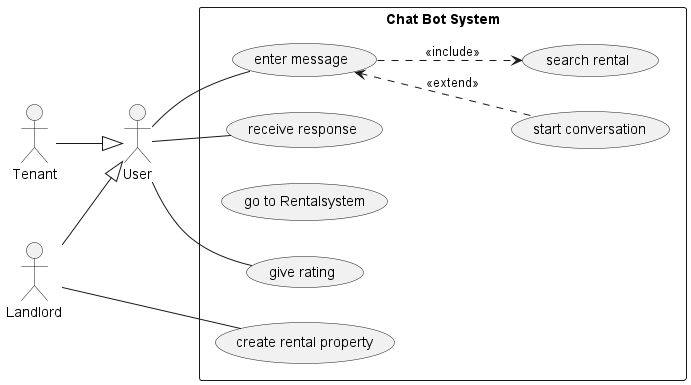
\includegraphics[width = \textwidth]{Images/chat_bot.png}
    \caption{Use Case diagram: AI chat-bot System}
    \label{fig:usecase-diagram-AI-system}
\end{figure}

\newpage
\subsubsection{Use case scenario}
\begin{table}[H]
    \centering
% \usepackage{tabularray}
\begin{longtblr}[
  label = none,
  entry = none,
]{
  width = \linewidth,
  colspec = {Q[125]Q[817]},
  hlines,
  vlines,
}
\textbf{Use-case ID}       & UC-11                              \\
\textbf{Use-case Name}     & Ask question     \\
\textbf{Actor(s)}          & User (Primary)                        \\
\textbf{Description}       & User can enter text to ask chat-bot system to search for specific characteristic rental post~~  \\
\textbf{Pre-condition(s)}  & User logged in successfully to the website                    \\
\textbf{Post-condition(s)} & Chat-bot system return closest results or responses               \\
\textbf{Trigger(s)}        & User clicks or focuses on the search input field                   \\
\textbf{Normal flow}       & {1. User inputs question in the chat box\\2. System processes and queries for the answer result\\3. System responses with an answer on the chat area\\4. System asks if the user wants to continue\\5. User wants to end the conversation\\End use case}  \\
\textbf{Alternative flow}  & {Alternative 1: At step 1 - User enter start conversation message instead of finding rental\\~1.1. User inputs start conversation message (e.g. Hello, Hi,...) \\~1.2. System responses with a greeting\\~1.3. System asks for the intent of user\\~1.4. User inputs question about rental finding\\~Continue at step 2 of the normal flow.
\\Alternative 2: At step 5: User want to ask more.
\\~Return to step 1 of the normal flow.~ ~} \\
\textbf{Exception flow}    & {Exception 1: at step 2 - System cannot understand the intent of Tenant, or Tenant enters value out of context of "finding rental" (e.g, "give me a sandwich")\\~Then the
system will ask again for more information with a guide message}
\end{longtblr}
    \caption{Use case scenario: enter message, receive response}
    \label{tab:usecase-scenario-enter-mess-&-resceive-response}
\end{table}


%-------UC-12-------------
\newpage
\begin{table}[H]
    \centering
% \usepackage{tabularray}
\begin{longtblr}[
  label = none,
  entry = none,
]{
  width = \linewidth,
  colspec = {Q[129]Q[813]},
  hlines,
  vlines,
}
\textbf{Use-case ID}       & UC-12                                  \\
\textbf{Use-case Name}     & Send feedback                          \\
\textbf{Actor(s)}          & User                                   \\
\textbf{Description}       & User send feedback after sending message with Chat-bot system                                        \\
\textbf{Pre-condition(s)}  & User sends message with the system and want to end conversation                                            \\
\textbf{Post-condition(s)} & Chat-bot system updates the feedbacks and to the database for future enhancement plan                     \\
\textbf{Trigger(s)}        & User want to end conversation after receiving response from system                                      \\
\textbf{Normal flow}       & {1. System ask if User wants to continue the conversation\\2. User wants to end the conversation\\3. System asks for rating and feedback\\4. User sends feedback\\5. System responses with the "Thank you!" message\\End use case} \\
\textbf{Alternative flow}  & Alternative 1: at step 2 - User enter new message after chat-bot system asks for feedback and rating. Then return to normal flow of~\textbf{\textbf{use-case UC-11}}      \\
\textbf{Exception flow}    & No exception                           \end{longtblr}
    \caption{Use case scenario: Send feedback}
    \label{tab:usecase-scenario-send-feed-back-AI}
\end{table}

%---------UC-13-----------
\newpage
\begin{table}[H]
    \centering
% \usepackage{tabularray}
\begin{longtblr}[
  label = none,
  entry = none,
]{
  width = \linewidth,
  colspec = {Q[148]Q[796]},
  hlines,
  vlines,
}
\textbf{Use-case ID}       & UC-13                            \\
\textbf{Use-case Name}     & Create rental inventory          \\
\textbf{Actor(s)}          & Landlord                          \\
\textbf{Description}       & Landlord can ask the chat-bot system to create rental inventory in the rental system automatically                                                 \\
\textbf{Pre-condition(s)}  & Landlord has logged in successfully                                                  \\
\textbf{Post-condition(s)} & Rental System create a rental post and adds it to the inventory list of landlord~           \\
\textbf{Trigger(s)}        & Landlord enters input field in chat-bot section with intent "create rental post"              \\
\textbf{Normal flow}       & {1. Landlord enter message\\2. Chat-bot system checks the message and get the all the required fields for a rental post from the message\\3. Chat-bot system prompts confirmation message to chat section\\4. Chat-bot system asks the Rental System to create a rental post and add it into inventory list\\5. Rental system routes to the detail page of the new rental property\\End use case} \\
\textbf{Alternative flow}  & {Alternative 1: At step 2 - The message is lack of some important information for a post (e.g, Price, Address, Image,...)\\~1.1 The chat-bot system asks for more information~\\~Return to step 1 in normal flow} \\
\textbf{Exception flow}    & No exception                     \end{longtblr}
    \caption{Use case scenario: Asking Chat-bot system to create rental property post}
    \label{tab:usecase-scenario-ask-chat-bot-create-rental}
\end{table}




\newpage
\section{Activity Diagrams}
From the use case scenarios, we can imagine the interaction flows between User and the System. But there are some constraints and requirements that we need to specify during the interaction processes between user and the application system, and these constraints can be demonstrated with the activity diagrams.
\subsection{Rental system: Authentication and Authorization}
Firstly, about Authentication and Authorization, there are several features that requires user account to use them. Moreover, because this is an application with goals are to recommend end-user their desire rentals and to connect with the rental owner, we need some validated and trustworthy contact information from the user, the solution is to ask the user to enter their phone number and email when signing up. If not, user can only access to some basic features of the system as guess, we made a table to show which feature user can access with or without an account:

\begin{table}[H]
    \centering
% \usepackage{tabularray}
\begin{longtblr}[
  label = none,
  entry = none,
]{
  width = 0.9\linewidth,
  colspec = {Q[115]Q[462]Q[200]Q[163]},
  row{1} = {c},
  cell{2}{1} = {r=8}{},
  cell{2}{3} = {c},
  cell{2}{4} = {c},
  cell{3}{3} = {c},
  cell{3}{4} = {c},
  cell{4}{3} = {c},
  cell{4}{4} = {c},
  cell{5}{3} = {c},
  cell{5}{4} = {c},
  cell{6}{3} = {c},
  cell{6}{4} = {c},
  cell{7}{3} = {c},
  cell{7}{4} = {c},
  cell{8}{3} = {c},
  cell{8}{4} = {c},
  cell{9}{4} = {c},
  cell{10}{1} = {c},
  cell{10}{3} = {c},
  cell{10}{4} = {c},
  vlines,
  hline{1-2,11} = {-}{},
  hline{3-10} = {2-4}{},
}
                  & \textbf{Feature}                           & \textbf{Without account} & \textbf{With account} \\
\textbf{Tenant }  & View rentals                               & \checkmark               & \checkmark            \\
                  & View rental details                        & \checkmark               & \checkmark            \\
                  & Search rental                              & \checkmark               & \checkmark            \\
                  & Compare 2 rentals                          & \checkmark               & \checkmark            \\
                  & Send message to Landlord                   &                          & \checkmark            \\
                  & Add rental to favorite/saved list          &                          & \checkmark            \\
                  & View saved list                            &                          & \checkmark            \\
                  & Give feedback                              &                          & \checkmark            \\
\textbf{Landlord} & * Every features in Landlord use case view &                          & \checkmark            
\end{longtblr}
    \caption{Accessing features with and without account}
    \label{tab:access-features}
\end{table}

\newpage
By this specification, we present the activity diagrams for Sign-up and Log-in as follow. The goals is to validated the user phone number and email to ensure the credibility of Landlord and communication between end-users.
\begin{figure}[H]
    \centering
    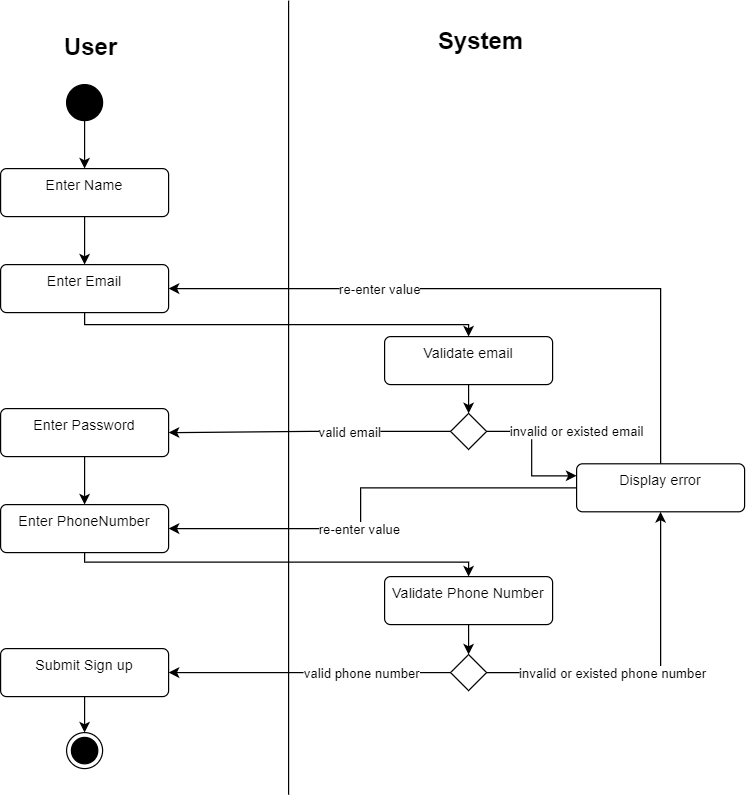
\includegraphics[width = 0.5\textwidth]{Images/Activity/ac_diag_signup.png}
    \caption{Activity diagram: Sign-up flow}
    \label{fig:signup-flow}
\end{figure}

\begin{figure}[H]
    \centering
    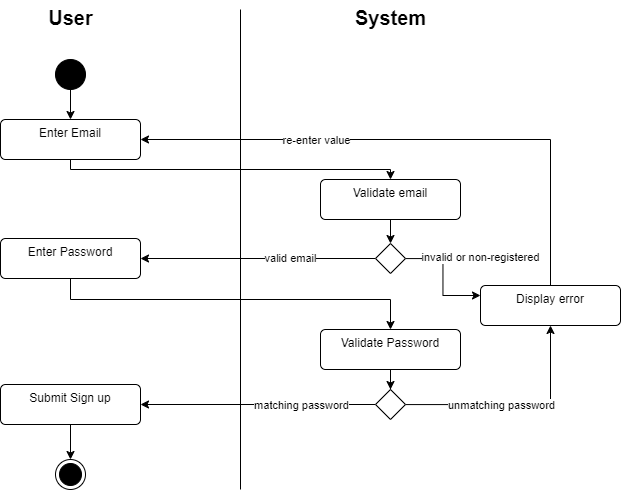
\includegraphics[width = 0.5\textwidth]{Images/Activity/ac_diag_login.png}
    \caption{Activity diagram: Log-in flow}
    \label{fig:login-flow}
\end{figure}

% ------AC_DIAG: TENANT-INTERACTION-------------
\newpage
\subsection{Rental system: Tenant interactions}
Secondly, about Tenant Module, there aren't many restrictions or constraints on the interaction between the Tenant and Rental system, the activity diagram are simply demonstrated the flow of interaction between the user and the system in general.

% -----AC-DIAG_VIew rental-------------
\subsubsection{Viewing the rentals on Tenant landing page or rental detail information page}
\begin{figure}[H]
    \centering
    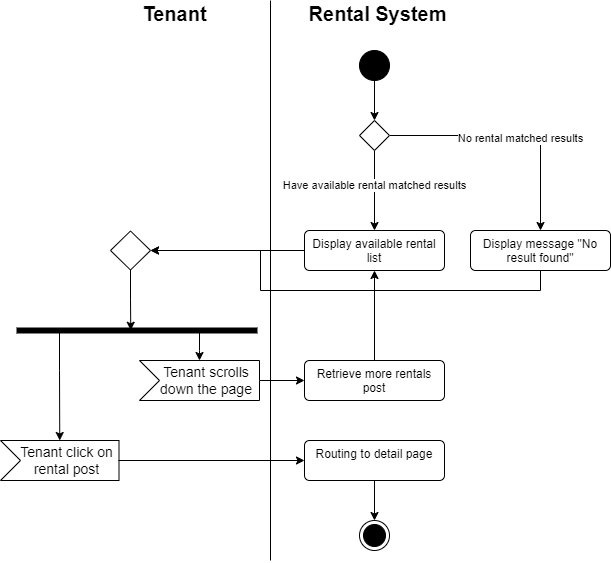
\includegraphics[width = 0.7\textwidth]{Images/Activity/ac_diag_view_rental.png}
    \caption{Activity diagram: Viewing rentals flow }
    \label{fig:ac_diag_view_rental}
\end{figure}

\noindent \textbf{Explanation:}\\
The activity diagram shows the flow when the user access to the website. First page of the website is the Landing page in Tenant view, so the user will be in the role of the Tenant who is looking for a house or an apartment for rent. The system retrieves the latest available rental system and display them with general rental detail to the Tenant.\\
There are two flows that the Tenant can follow. If the Tenant keeps scrolling down for more rentals, then the Rental system will retrieve for more rentals and display them to the page. If the Tenant clicks on a rental post - meaning he/she want to see more detail information about that rental, then the System will retrieve the detail information and redirect the Tenant to the Detail Information page


% -----AC-DIAG_comparing rental-------------
\newpage
\subsubsection{Comparing 2 rentals}
\begin{figure}[H]
    \centering
    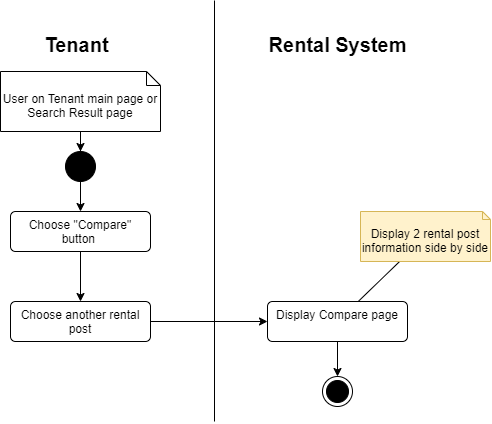
\includegraphics[width=0.8\textwidth]{Images/Activity/ac_diag_compare_2_rentals.png}
    \caption{Activity diagram: Comparing rentals flow}
    \label{fig:compare-rentals}
\end{figure}
\noindent \textbf{Explanation:}\\
The activity diagram describes the flow when the Tenant want to compare 2 rental post. The Tenant is viewing the list of available rentals, he/she can clicking on "Comparison" button on a rental post in the list. The next step is that the System will ask the Tenant to choose another post. Then the Tenant choose another post for starting the comparison or he/she can cancel the comparison process (if the Tenant hit on "Cancel" button, the System will stop asking for the second rental post and let the Tenant continue the Viewing rentals flow). After getting 2 rentals, the System will redirect to the comparison page and display the detail information side by side.


% -----AC-DIAG_searching rental-------------
\subsubsection{Searching rentals}
\begin{figure}[H]
    \centering
    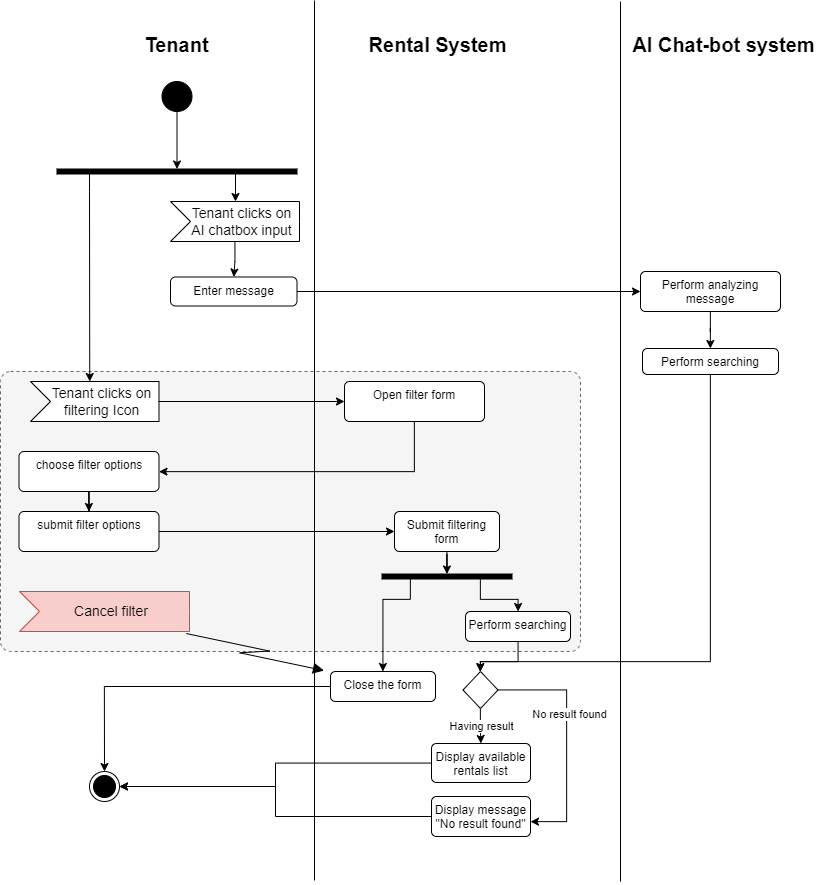
\includegraphics[width=0.7\textwidth]{Images/Activity/ac_diag_search_rental.png}
    \caption{Activity diagram: Searching rentals}
    \label{fig:searching-rentals}
\end{figure}
\noindent \textbf{Explanation:}\\
The activity diagram describes the flows when the Tenant want to search for the rentals based on their criteria. There are 2 ways to help the Tenant achieving their goal: by entering message or by opening the filter.\\
If the Tenant chooses to search by filtering, the System then opens a filtering form so that the Tenant can click and choose the criteria he/she wants (e.g, Property Type, Price Range, Number of rooms, Dimensions,...). Then after the Tenant done choosing and hit the "Save" button, the System can perform searching for the rentals and display the result to the Tenant.\\
If the Tenant chooses to search by entering message, he/she can just enter a message into search input, then a dialog box will be opened and the System can use the Chat-bot AI system to help parsing the message, getting the intent and also the criteria from the user. Then the System performs searching and display the result to the user.


% -----AC-DIAG_adding rental to favorite lsit-------------
\newpage
\subsubsection{Adding rental to favorite list}
\begin{figure}[H]
    \centering
    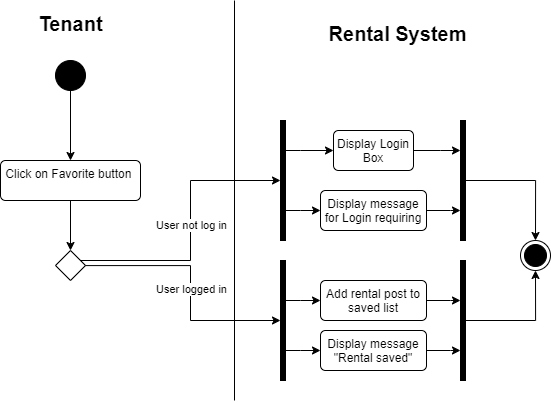
\includegraphics[width=0.8\textwidth]{Images/Activity/ac_diag_add_favorite.png}
    \caption{Activity Diagram: Adding to favorite list}
    \label{fig:add-favorite}
\end{figure}
\noindent \textbf{Explanation:}\\
The activity diagram describes the flows when user saves the rental to his/her favorite list for the later reviewing. The Tenant can click on the "Favorite" button which means he/she want the system to add this rental post into the favorite list. As we mentioned earlier, this feature can only be accessed when User has an account on the website. Therefore, when clicking on the "Favorite" button, the System will perform checking if the User had accessed to the website by Guess account or by his/her account. Then there are 2 case might happen.\\
If the Tenant uses the Guess account, the System displays a Log-In Box with a message, telling the Tenant that they might want to login to use this feature.\\
If the Tenant uses his/her account, the System will perform adding the rental to the favorite list of that account. After adding the post, the System displays a confirmation message to the Tenant 



% _____LANDLORD INTERACTION_____________
\newpage
\subsection{Rental system: Landlord interactions}
Thirdly, about Landlord Module, this allows the User to create, update, delete their rentals inventories. Because the goal is to check and maintain the reliability and the trustworthiness of the rentals and the house owners, these features require the User to log in the website so that they can use them. 
% ----AC_Diag: View rentals-----------
\subsubsection{Viewing rental inventories}
\begin{figure}[H]
    \centering
    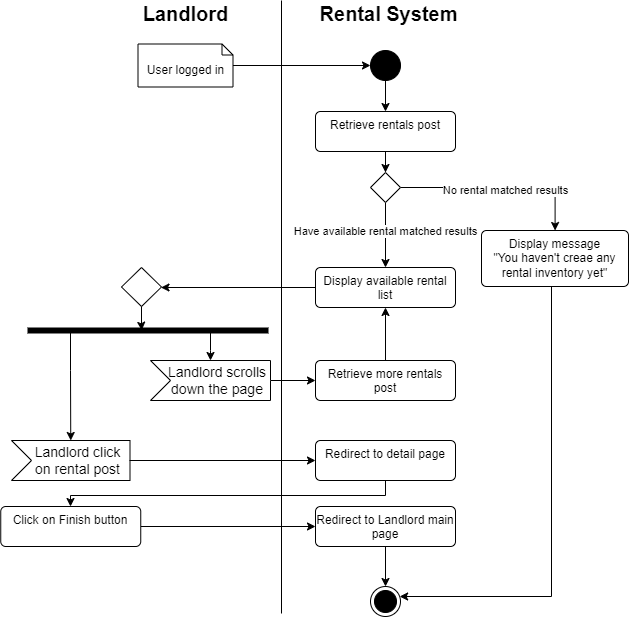
\includegraphics[width=0.9 
    \textwidth]{Images/Activity/ac_diag_view_landlord.png}
    \caption{Activity diagram: Viewing rental inventories}
    \label{fig:viewing-rental-landlord}
\end{figure}
\noindent \textbf{Explanation:}\\
The activity diagram describes the flow of viewing the rental properties when the User changes from Tenant View into Landlord view. When the User clicks on "Landlord" button, he/she will be redirected to Landlord Landing page. The system will retrieve all rental inventories (the rental post that the Landlord had created) and display it on the page. If the Landlord haven't create any rental inventory, the system will display the message onto the page. \\
There are 2 flow that the Landlord can follow. If the Landlord keeps scrolling down for more rentals, then the Rental system will retrieve for more rental inventories and display them to the page from the newest to the oldest rental creation date. If the Landlord clicks on a rental post - meaning he/she want to see more detail information about that rental, then the System will retrieve the detail information and redirect the Tenant to the Detail Information page. After done viewing the detail information, the Landlord can click on "Return" button to return to the Landlord Landing page. 


% -----AC_Diag: Create rental---------
\newpage
\subsubsection{Creating rental inventory}
\begin{figure}[H]
    \centering
    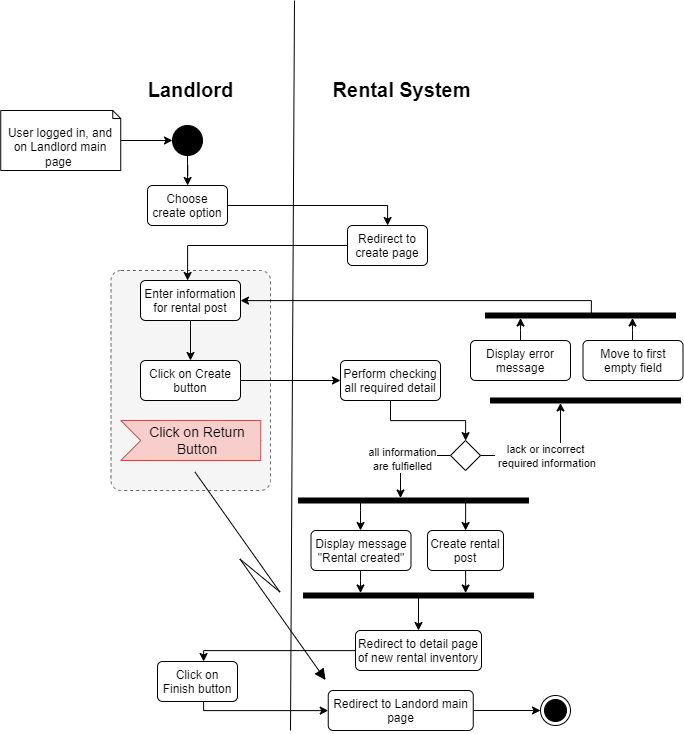
\includegraphics[width=0.7\textwidth]{Images/Activity/ac_diag_create_rental_post_manual.png}
    \caption{Activity diagram: Creating rental property}
    \label{fig:create-rental}
\end{figure}
\noindent \textbf{Explanation:}\\
The activity diagram describes the flow when the Landlord creates a new rental inventory. The system will then redirect the Landlord to the Create page. Then the Landlord can start adding information for his rental inventory.\\
The Landlord can cancel the creating process anytime by clicking on the "Return" button. Then, the System will return on the Landlord Landing page.\\
Because we must keep a rental post reliable, there are some information that is required (address, price, image, owner's phone number)  After the Landlord hit on the "Create" button, the System will check if all required information are fulfilled. If not, the System will display an alert and jump to the information that is invalid for the re-entering. If all information are fulfilled, the System can create a rental post and then redirect the Landlord to the rental detail page of the new rental inventory.

%-------Ac-diag: Update rental--------
\newpage
\subsubsection{Updating rental property}
\begin{figure}[H]
    \centering
    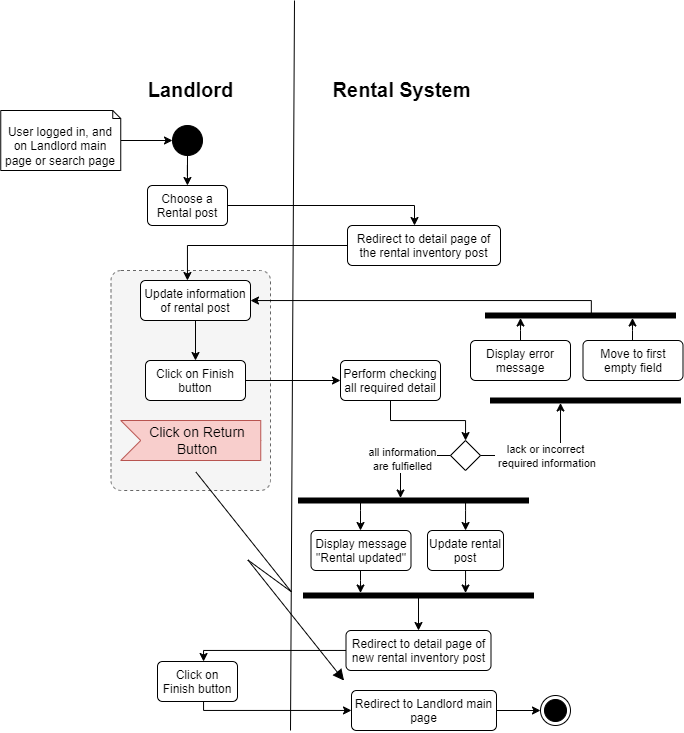
\includegraphics[width=0.7\textwidth]{Images/Activity/ac_diag_update_rental.png}
    \caption{Activity diagram: Updating rental property}
    \label{fig:update-rental}
\end{figure}
\noindent \textbf{Explanation:}\\
The activity diagram describes the flow when the Landlord updates an existing rental inventory. This flow is the same as the "Creating rental inventory flow" but instead of clicking the "Create" button, the Landlord will choose a post in the rental inventory list in Landing page. The system will open the Detail information page of that rental post and the Landlord can start updating the information. The information checking flow and cancelling is almost the same as the "Creating" flow. The system still has to check and ensure that there is no rental information is invalid.


%-------Ac-diag: Delete rental--------
\newpage
\subsubsection{Deleting rental property}
\begin{figure}[H]
    \centering
    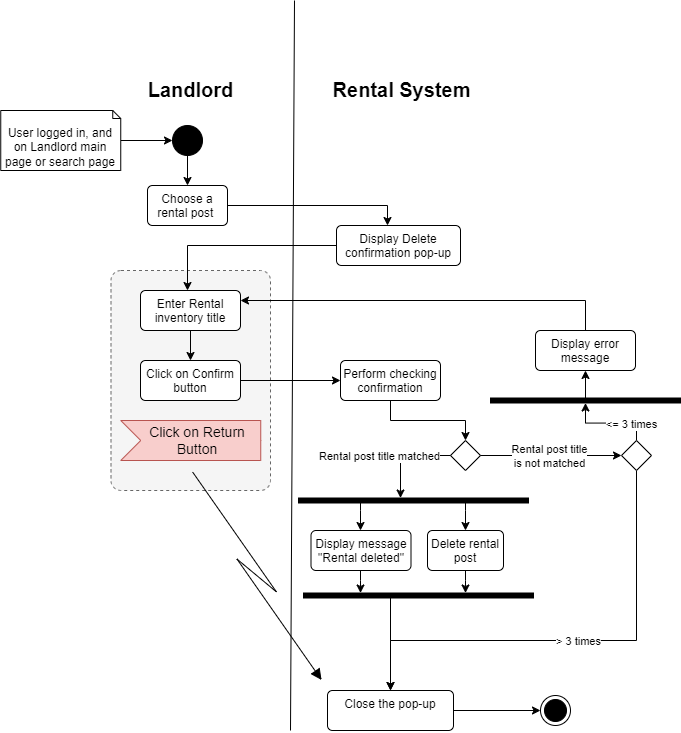
\includegraphics[width=0.7\textwidth]{Images/Activity/ac_diag_delete_post.png}
    \caption{Activity diagram: Deleting rental property}
    \label{fig:delete-rental}
\end{figure}
\noindent \textbf{Explanation:}\\
The activity diagram describes the flow when the Landlord deletes the rental property. When the Landlord want to delete a rental property, he/she can click on the "Delete" button on the rental post if the User is viewing the rentals list or on the Detail information page of a specific rental post.\\
To ensure that the User does not accidentally delete the rental property, the System will display a pop-up that require the Landlord to enter the title of that rental inventory, and also a confirmation message including the rental title (the purpose is to give the owner of the property have time to reconsidering the deletion, not to make the extra step to make it hard to use). \\
Next, the System start checking if the entered title is matching with the actual title or not. If not, the User has 3 tries to enter the correct title, more than 3 times will cause the System cancel the deletion process. After the Landlord entered the correct value, the System will delete the rental post. \\
Moreover, the Landlord cancel the deletion process at anytime.


\newpage
\subsection{Chat-bot system: User interactions}
Finally, about the Chat-bot AI System, the main purpose of the Chat-bot system is to enhance the experience of the User by improving the searching and creating the rental post.
% -----Ac-Diag: Searching chat-bot--------------------
\subsubsection{Interacting with Tenant}
\begin{figure}[H]
    \centering
    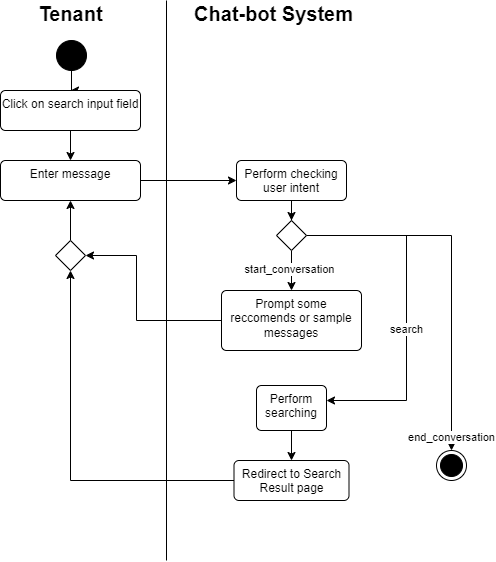
\includegraphics[width=0.9\textwidth]{Images/Activity/ac_diag_search_by_chat_bot.png}
    \caption{Activity diagram: Interaction with Tenant}
    \label{fig:Interaction-with-Tenant}
\end{figure}
\noindent \textbf{Explanation:}\\
The activity diagram describes in more detail the flow when the User search for rental by entering message. The System will receive the message from the User, then it has 3 option to continue the flow.
\begin{itemize}
    \item If the Tenant want to start the conversation, the System will answer with some instruction about how to perform searching with a message.
    \item If the Tenant want to search for rental, the System will get all the criteria from the message and the Rental System will perform searching based on the criteria got from the Chat-bot.
    \item If the Tenant want to end the conversation, the Chat-bot system will display thank you message and ask for the feedback.
\end{itemize}


% -----Ac-Diag: Creating chat-bot--------------------
\newpage
\subsubsection{Interacting with Landlord}
\begin{figure}[H]
    \centering
    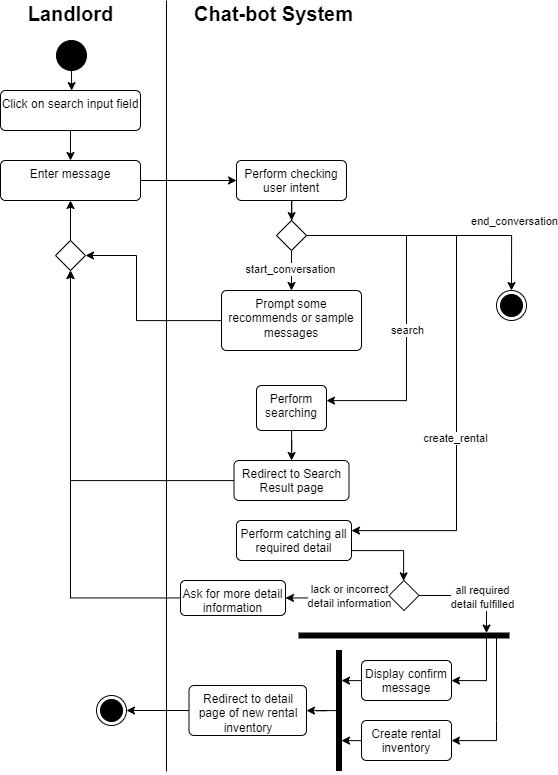
\includegraphics[width=0.8\textwidth]{Images/Activity/ac_diag_create_rental_chat_bot.png}
    \caption{Activity diagram: Interacting with Landlord}
    \label{fig:Interacting-with-Landlord}
\end{figure}
\noindent \textbf{Explanation:}\\
The activity diagram describes in more detail the interaction flow between the Landlord and the Chat-bot system. The System will receive the message from the User, then it has 4 options to continue the flow. There are 3 options that are similar to the interaction flow of the Tenant, but the Landlord interaction has 1 more option which is "Creating rental inventory"\\
\begin{itemize}
    \item If the Landlord want to start the conversation, the System will answer with some instruction about how to perform searching with a message.
    \item If the Landlord want to search for rental, the System will get all the criteria from the message and the Rental System will perform searching based on the criteria got from the Chat-bot and display the result to the Landlord.
    \item If the Landlord want to end the conversation, the Chat-bot system will display thank you message and ask for the feedback.
    \item If the Landlord want to create a new rental inventory, the Chat-bot system will retrieve all information from the message for the new rental inventory. Again, if the required information are not fulfilled, the System need to send the message asking the user to enter more information until it can make a new rental inventory. After the creation process, the Landlord will be redirect to the Detail page of the new rental inventory.
\end{itemize}


% ######### SEQUENCE DIAGRAM ########
\newpage
\section{Sequence diagrams}
\subsection{Tenant Interaction}
\subsubsection{Viewing rental and rental detail}
\begin{figure}[H]
    \centering
    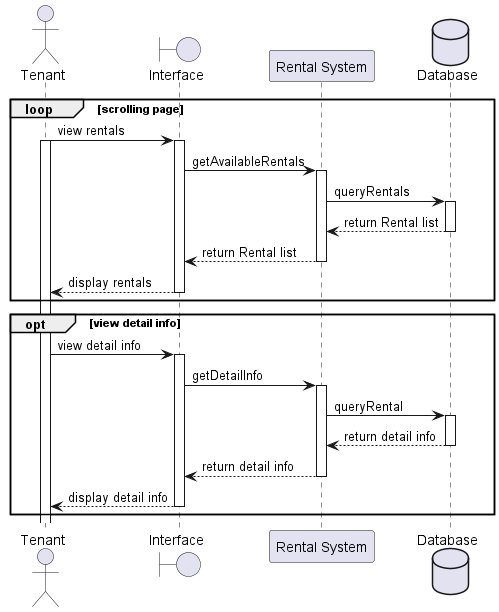
\includegraphics[width=0.7\textwidth]{Images/Sequence/seq_diag_view_rental.png}
    \caption{Sequence diagram: view rental and rental detail}
    \label{fig:seq-diag-view-rental}
\end{figure}
\noindent \textbf{Explanation:}\\
The sequence diagram explains how the Tenant can see the rental on the website. In this context, the Interface in the diagram refers to the User Interface, but we will named it "Interface" for short. When the Tenant is on the Tenant Landing page, the Interface need the list of available rentals to show to the Tenant. Therefore, the Rental System will retrieve rental from the Database. After the Database return the result, the System will display them to the User through the Interface.


\newpage
\subsubsection{Comparing rentals}
\begin{figure}[H]
    \centering
    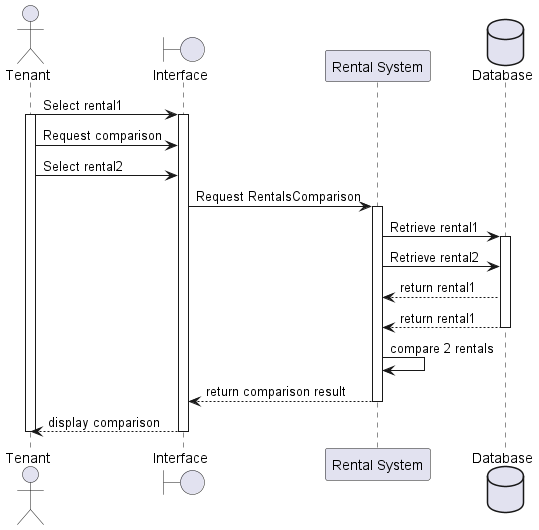
\includegraphics[width=0.8\textwidth]{Images/Sequence/compare_rental.png}
    \caption{Sequence diagram: Comparing 2 rentals}
    \label{fig:seq-diag-compare}
\end{figure}
\noindent \textbf{Explanation:}\\
The sequence diagram shows how the Tenant can compare 2 rentals but the idea of the flow is already described in the activity diagram. After Tenant clicked on the "Compare" button on a rental post and chose the second rental post, this mean it issues the rental comparison feature of the Rental System. The System will based on the 2 chosen rental post to retrieve more information from the Database, then rearranged the information in the way that the Interface can display these detail information side by side to the Tenant. 


\newpage
\subsubsection{Searching rental}
\begin{figure}[H]
    \centering
    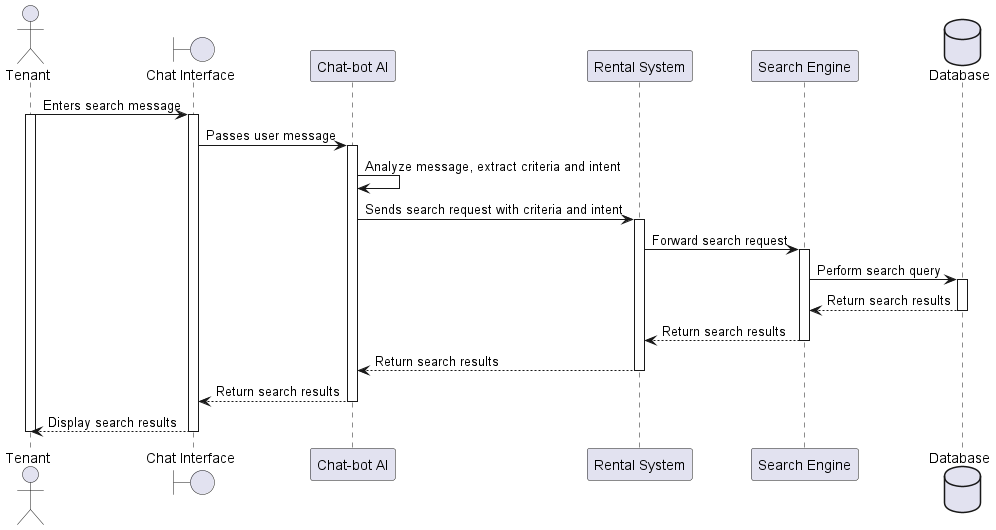
\includegraphics[width=0.9\textwidth]{Images/Sequence/seq_diag_search.png}
    \caption{Sequence diagram: Searching rentals}
    \label{fig:seq-diag-search}
\end{figure}
\noindent \textbf{Explanation:}\\
The sequence diagram describes how the Tenant can perform searching for the rentals. The Tenant enters the message to search through the Interface, and the Chat-bot System is responsible for handling the message. The handling message process includes analyze, extract all criteria and detect the intent from the message, and pass them to the Rental System. Next, the System will use the Search Engine and the information to query form the Database. After the Database returns the result, the Rental System will passed it to the Chat-bot System so it can create a message and responses to the User. 



\newpage
\subsubsection{Saving and viewing favorite list}
\begin{figure}[H]
    \centering
    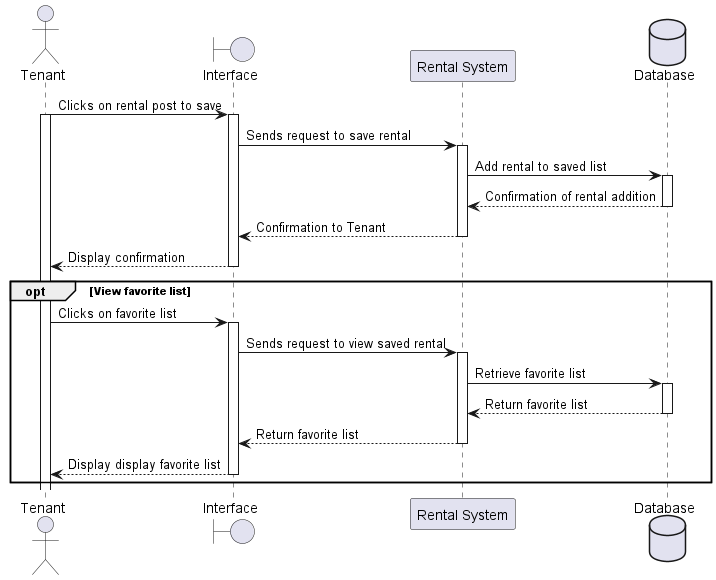
\includegraphics[width=0.8\textwidth]{Images/Sequence/seq_diag_save_&_view_saved_rental.png}
    \caption{Sequence diagram: Saving and viewing favorite list}
    \label{fig:seq-diag-favorite}
\end{figure}
\noindent \textbf{Explanation:}\\
The sequence diagram describe how the Tenant can save and might view the favorite list. The sequence is the same as the flow described in the Activity diagram. When the user clicks on the "Save" button on a rental post, the System can update the rental post to the Database, and then confirm back to the User if success.


\newpage
\subsection{Landlord Interaction}
\subsubsection{Creating rental with the Interface}
\begin{figure}[H]
    \centering
    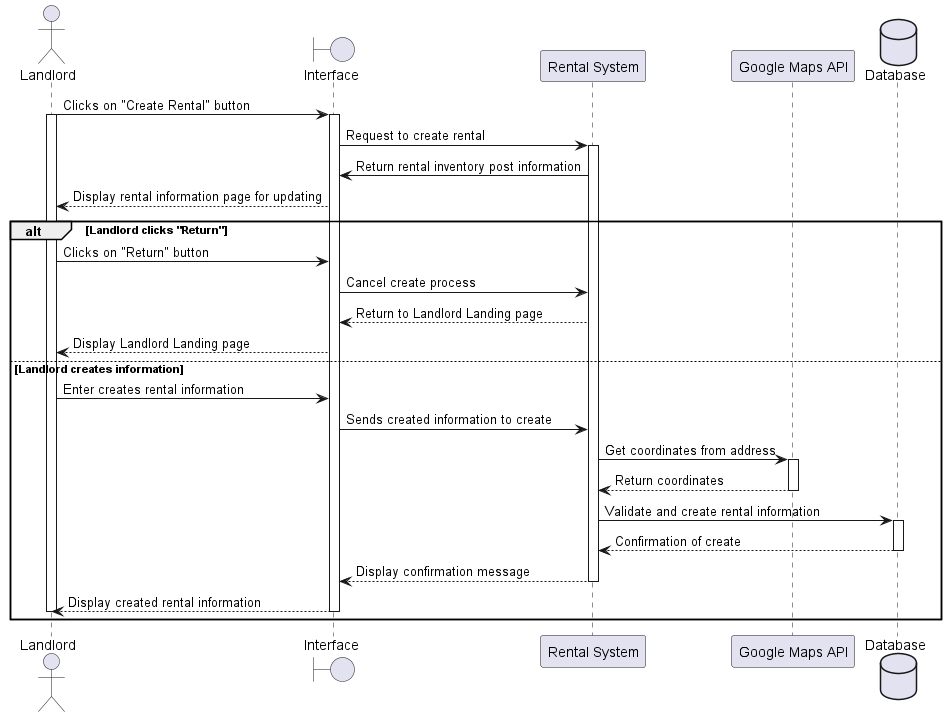
\includegraphics[width=0.9\textwidth]{Images/Sequence/seq_diag_create_rental_inventory.png}
    \caption{Sequence diagram: Creating rental with the Interface}
    \label{fig:seq-diag-create-chat-bot}
\end{figure}
\noindent \textbf{Explanation:}\\
The sequence diagram illustrates how landlord create a new rental inventory. The sequence has the similar flow described in the activity diagram, except there is an extra step before the System tell the Database to create a new rental. Because we need to get the coordinates of the rental for the business logic, the System need to call Google API to get the coordinates from the address, then the System can tell the Database to create a new rental for the Landlord.


\newpage
\subsubsection{Creating rental with Chat-bot system}
\begin{figure}[H]
    \centering
    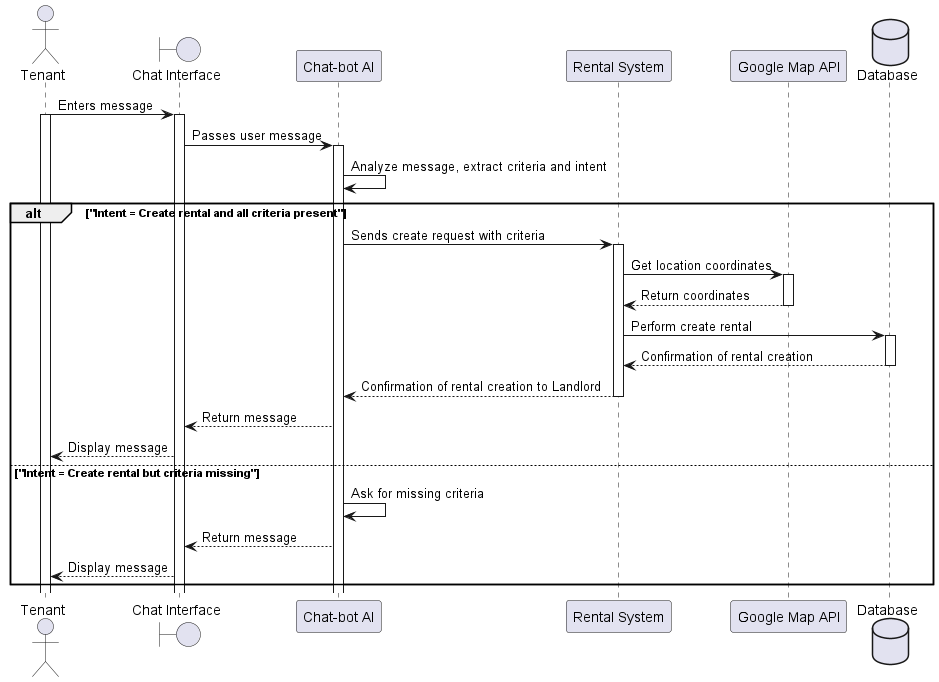
\includegraphics[width=0.9\textwidth]{Images/Sequence/seq_diag_create_rental_inventory_bot.png}
    \caption{Sequence diagram: Creating rental with Chat-bot system}
    \label{fig:seq-diag-create-chat-bot}
\end{figure}
\noindent \textbf{Explanation:}\\
The sequence diagram illustrated how the Landlord can create a new rental inventory, but this time with the help of the Chat-bot system. Instead of entering the information in the fields on the page, the Landlord now enters a message to the Chat-bot so it can analyze the intent of the Landlord and the criteria in the message. If the message does not contains enough information for the creation process than the Chat system can generate the response to ask for more information.
Consequently, if all information are fulfilled then the Chat System can pass them to the Rental System. Here, the next steps is similar to the sequence happened when the Landlord create a new rental with the User Interface.



\newpage
\subsubsection{Updating rental information}
\begin{figure}[H]
    \centering
    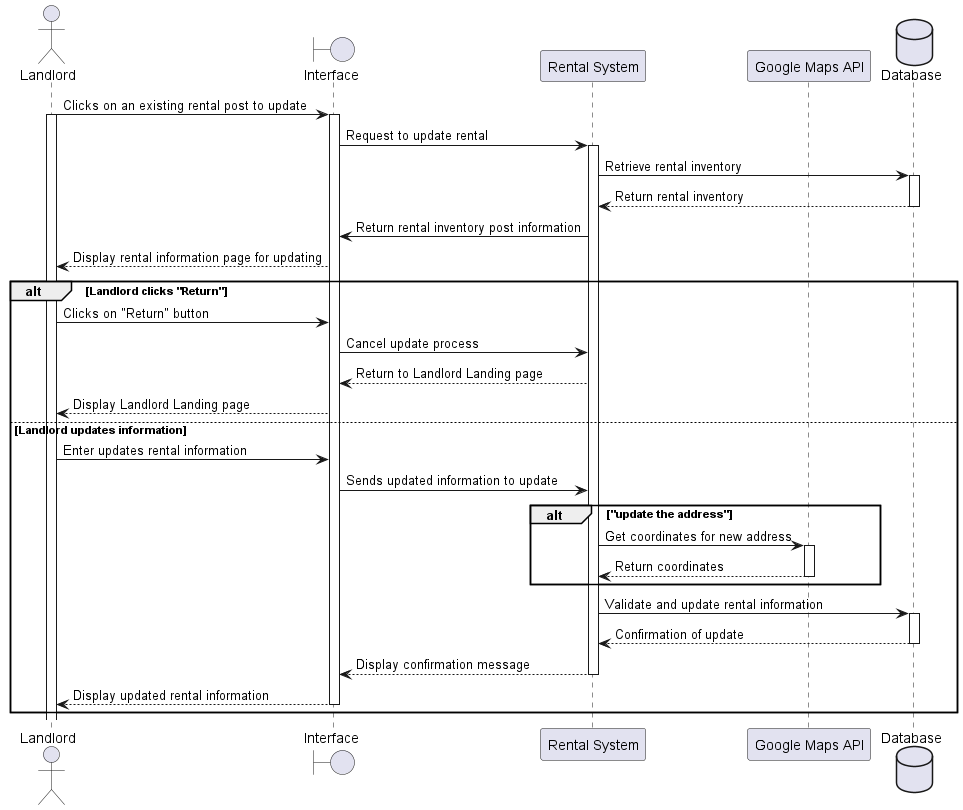
\includegraphics[width=0.9\textwidth]{Images/Sequence/seq_diag_update_rental_inventory.png}
    \caption{Sequence diagram: Updating rental inventory}
    \label{fig:update-rental}
\end{figure}
\noindent \textbf{Explanation:}\\
The sequence diagram describes how the Landlord can update the information of a specific rental inventory. The flow is also described in the activity diagram, this sequence diagram only explains more about the actions of the Rental System when it retrieves and process the detail information from the Database to display to the Landlord; or when the System need to call the API from Google Maps to derive the coordinates of the address of the rental (if the User updates a new address) before it perform updating to the Database.


\newpage
\subsubsection{Deleting rental inventory}
\begin{figure}[H]
    \centering
    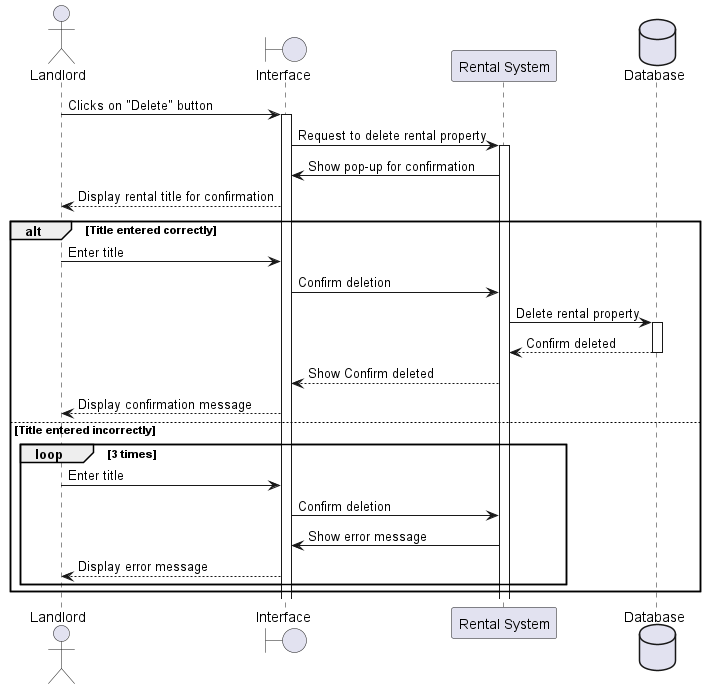
\includegraphics[width=0.8\textwidth]{Images/Sequence/seq_diag_delete_rental_inventory.png}
    \caption{Caption}
    \label{fig:enter-label}
\end{figure}
\noindent \textbf{Explanation:}\\
The sequence diagram illustrates the message exchanged when the Landlord deletes an existing rental inventory. This flow is also similar to the flow described in the corresponding activity diagram. The Landlord click on the "Delete" button when he/she decides to delete this rental. This event issue the Rental System to open a pop-up that require the User to confirm the deleting. Then, the System can check to confirmation and continue to delete the rental inventory.